\documentclass[11pt]{amsart}
\usepackage{amsmath,amsthm,amsfonts,amssymb,enumerate}
\usepackage[normalem]{ulem}
\usepackage{ dsfont }
\usepackage{geometry}
\usepackage{graphicx}
\usepackage{float}


\title{Convex and Nonsmooth Optimization:\\HW 5}
\author{Terrence Alsup}
\date{March 10, 2020}

\begin{document}
\maketitle
\begin{enumerate}
%%%%%%%%%%%%%%%%%%%%%%%%%%%%%%%%%%%%%%%%%%%
\item \begin{enumerate}

\item The Matlab function \texttt{gradmeth.m} contains the gradient method implementation and the Matlab function \texttt{linesearch.m} implements backtracking linesearch that returns the step length to take.  After 100 iterations of gradient descent on the example problem ($A$ is the badly conditioned Hilbert matrix) we compute that
\[
\frac{f(x^{(k)}) - p^*}{f(x^{(0)}) - p^*} \approx 0.31
\]
where $x^{(0)} = (1,1,1,1,1)^T$.  Here we compute that the true optimal value is $p^* = -12.5$.  Since this problem is quadratic, the Hessian $\nabla^2 f(x) = A$, which has smallest and largest eigenvalues
\[
m = \lambda_{\min}^A \approx 3.29 \times 10^{-6},\quad M = \lambda_{\max}^A \approx 1.57
\]
The condition number of this matrix is very large and
\[
c = 1 - \frac{m}{M} \approx 1 - 2.098 \times 10^{-6}
\]
is very close to 1.  The theory says that after 100 iterations
\[
\frac{f(x^{(k)}) - p^*}{f(x^{(0)}) - p^*} \le c^{100} \approx 0.9979
\]
which is almost no improvement.  However, this is only an upper bound and in fact we saw that for our starting point gradient descent actually does much better initially (and hence still obeys the upper bound).  One more note is that this slow convergence is actually observed if the number of iterations is increased.


\item For the optimization problem in Boyd and Vandenberghe, the objective function is
\[
f(x) = -\sum_{i=1}^m \log(1 - a_i^Tx) - \sum_{i=1}^n \log(1 - x_i^2)
\]  
when $a_i^T x < 1$ for $i=1,\ldots,m$ and $|x_i| < 1$ for $i=1,\ldots,n$.  The partial derivatives that define the gradient are
\[
\frac{\partial}{\partial x_j}f(x) = \sum_{i=1}^m \frac{a_{ji}}{1 - a_i^Tx} + \frac{2x_j}{1 - x_j^2}
\]
The objective function as well as its gradient and Hessian (for Newton's method later) are implemented in the Matlab function \texttt{objective\_fun.m}.  We check that the gradient is implemented correctly by comparing with the finite difference values of $f(x)$, which is implemented in the Matlab script \texttt{FDcheck.m}.  The results in the figure below show that the implementation is indeed correct.

\begin{figure}[H]
\centering
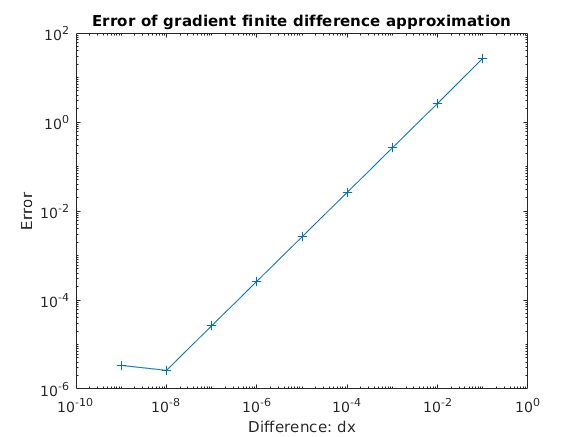
\includegraphics[width=5in]{grad_fd.png}
\caption{The error of the finite difference approximations to the gradient.}
\label{fig:grad_fd}
\end{figure}


We now run the gradient method implementation on this problem and find that it takes 70 iterations to achieve a tolerance of $10^{-6}$ and we get
\[
p^* \approx -67.463721
\]
Figure~\ref{fig:error} below (in part 2b) shows the values of $f(x^{(k)}) - p^*$ for $k = 1,\ldots,69$ (we do not plot the last iteration since it would be 0) for the gradient method.  Similarly, the norms of the gradients $\|\nabla f(x^{(k)})\|_2$ are plotted in Figure~\ref{fig:gradnorms}.  We can also estimate the condition number $M/m$ using this data.  We know that
\[
\frac{f(x^{(k)}) - p^*}{f(x^{(0)}) - p^*} \le c^k
\]
where $c = 1 - \frac{m}{M}$.  Taking the log of both sides gives
\[
\log \left[ \frac{f(x^{(k)}) - p^*}{f(x^{(0)}) - p^*} \right] \le k\log c = k\log \left( 1 - \frac{m}{M} \right)
\]
Since this bound should hold for all iterations $k$ we estimate $\log c$ by
\[
\log c = \max_{k} \frac{1}{k} \log \left[ \frac{f(x^{(k)}) - p^*}{f(x^{(0)}) - p^*} \right] 
\]
and from here we estimate the condition number by $\frac{M}{m} = (1 - e^{\log c})^{-1} \approx 2.569$.  The Matlab script used to run the gradient method (and Newton's method) for this problem is \texttt{BV\_problem.m}.  The same script also plots the results and estimates the condition number.

\end{enumerate}
%%%%%%%%%%%%%%%%%%%%%%%%%%%%%%%%%%%%%%%%%%%

\vspace{0.5in}

%%%%%%%%%%%%%%%%%%%%%%%%%%%%%%%%%%%%%%%%%%%

\item 

\begin{enumerate}

\item To solve the quadratic problem
\[
\min f(x) = \frac{1}{2}x^TAx + x^Tb
\]
with Newton's method is trivial because it only needs 1 iteration.  The gradient is $\nabla f(x) = Ax + b$ and the Hessian is $\nabla^2 f(x) = A$.  Thus, the Newton search direction is 
\[
-A^{-1}(Ax + b) = -x - A^{-1}b
\]
and therefore, after the Newton update we are just left with $-A^{-1}b$, which is exactly the optimal solution.




\item The implementation of Newton's method is in the Matlab function \texttt{newtmeth.m}.  For the Hessian of the objective function, we compute that the second partial derivatives are given by
\[
\frac{\partial^2}{\partial x_j \partial x_k} f(x) = \sum_{i=1}^m \frac{a_{ji}a_{ki}}{(1 - a_i^Tx)^2} + 2\left( \frac{1 + x_j^2}{(1 - x_j^2)^2}  \right) \delta_{jk}
\]
where $\delta_{jk} = 1$ if $j = k$ and is 0 otherwise.  The same script, \texttt{FDcheck.m}, that was used to check the gradient also checks the Hessian using finite differences of the gradients.  The figure below shows that the implementation of the Hessian is indeed accurate.

\begin{figure}[H]
\centering
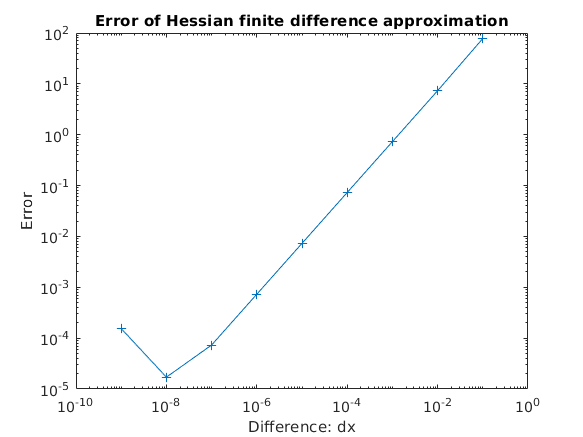
\includegraphics[width=5in]{hess_fd.png}
\caption{The error of the finite difference approximations to the Hessian.}
\label{fig:grad_fd}
\end{figure}

The Matlab script \texttt{BV\_problem.m} runs Newton's method on the problem.  The results for both Newton's method and the gradient method are in the two figures below.  Indeed we see that Newton's method converges quadratically.  Although Newton's method runs for 20 iterations, it really only takes about 6-7 iterations to reach a very small error (near machine precision).  In order to compare this with the theoretical number of iterations needed we need to estimate the values $m,M,L$.  For this purpose, we take an eigenvalue decomposition of the Hessian at every iteration and set $m$ to be the smallest and $M$ to be the largest eigenvalues over all of the iterations.  Similarly, we estimate the Lipschitz constant $L$ by taking the max
\[
L = \max_k \frac{\| \nabla^2 f(x^{(k)}) - \nabla^2 f(x^{(0)})  \|_2}{\|x^{(k)} - x^{(0)}\|_2}
\]
We estimate that $m \approx 2$, $M \approx 281.6$ and $L \approx 210.3$.  Using these values we see that the condition number of the problem is approximately $M/m \approx 140$, which means that the estimate from the gradient method was a significant underestimate.  The upper bound for the number of Newton iterations is given by
\[
\frac{f(x^{(0)}) - p^*}{\gamma} + \log_2 \log_2 \frac{2m^3}{\epsilon L^2}
\]
and $\gamma = \alpha \beta \eta^2 \frac{m}{M}$, where $\alpha = 0.25, \beta = 0.5$, and $\eta = \min \{ 1, 3(1 - 2\alpha)\} \frac{m^2}{ L}$.  Computing these values gives an extremely large upper bound
\[
\text{\# Newton iterations  } \le 210,109,870 \approx 2.1 \times 10^8
\]
iterations.  Obviously this bound is very loose because the algorithm performs much better in practice.



\begin{figure}[H]
\centering
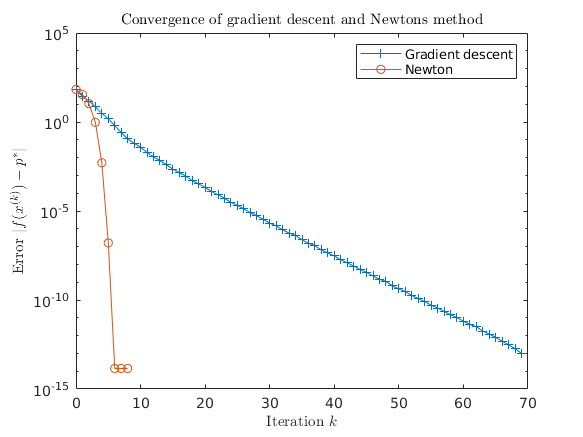
\includegraphics[width=5in]{error.png}
\caption{The error $|f(x^{(k)}) - p^*|$ for both Newton's method and the gradient method.}
\label{fig:error}
\end{figure}


\begin{figure}[H]
\centering
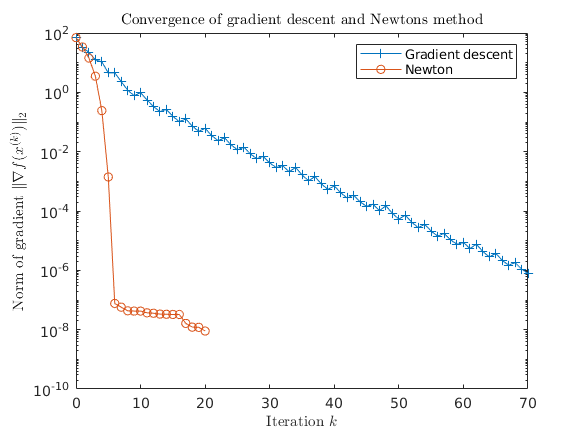
\includegraphics[width=5in]{gradnorms.png}
\caption{The norms of the gradients $\|\nabla f(x^{(k)})\|_2$ for both Newton's method and the gradient method.}
\label{fig:gradnorms}
\end{figure}

\end{enumerate}


%%%%%%%%%%%%%%%%%%%%%%%%%%%%%%%%%%%%%%%%%%%





\end{enumerate}

\end{document}